\documentclass[14pt, a4paper]{extreport}
\usepackage{susu}

% ====================================================================================================
\begin{document}

\author{Савонин~М.В.}
\group{211}
\task{5}
\maketitle

% ====================================================================================================
\chapter{Задание}

\begin{enumerate}

	\item
	Написать программу для построения гладкой кривой по четырем опорным точкам. При выборе опорных точек текущие координаты указателя мыши 	должны отображаться в графическом окне. Интерфейс программы должен содержать следующие элементы управления:
	\begin{itemize}
		\item выбор опорных точек;
		\item построение кубической кривой Безье;
		\item построение кривой по алгоритму Чайкина;
		\item сохранение результата в файл;
		\item выход из программы.
	\end{itemize}

\end{enumerate}

% ====================================================================================================
\chapter{Математическая модель}

\MakeUppercase{Кривая Безье}\\
Пусть $x_i$, $y_i$ одна из n точек кривой.
Находим треугольник Паскаля и берём строку номер n в массив pasc.\\
Проходимя от t=0 до 1 с шагом step.\\
Проходим от i=0 до i<n с шагом 1.\\
рисуем линию от предыдущей точки до точки:
$$ x = pasc_{i}*(1-t)^{n-i-1}*t^{i}*x_i .$$
$$ y = pasc_{i}*(1-t)^{n-i-1}*t^{i}*y_i .$$\\
\\
\MakeUppercase{Кривая Чайкина}\\
Берём первые 2 точки, находим на отрезке между ними 1/4 и 3/4 и забываем предыдущие.\\
Потом берём 2 и 3 точку и выполняем те же действия до последней точки.\\
Выполняем эти действия 5 раз для получившихся точек.\\
рисуем линии от точки к точки по получившимся точкам.

% ====================================================================================================
\chapter{Текст программы}

\noindent Файл main.cpp
\lstinputlisting{source/main.cpp}
\pagebreak
\hrulefill

\noindent Файл draw.h
\lstinputlisting{source/draw.h}
\hrulefill

\noindent Файл draw.cpp
\lstinputlisting{source/draw.cpp}
\hrulefill

\noindent Файл control.h
\lstinputlisting{source/control.h}
\hrulefill

\noindent Файл control.cpp
\lstinputlisting{source/control.cpp}

% ====================================================================================================
\chapter{Результат работы}

\begin{figure}[h!]
	\centering
	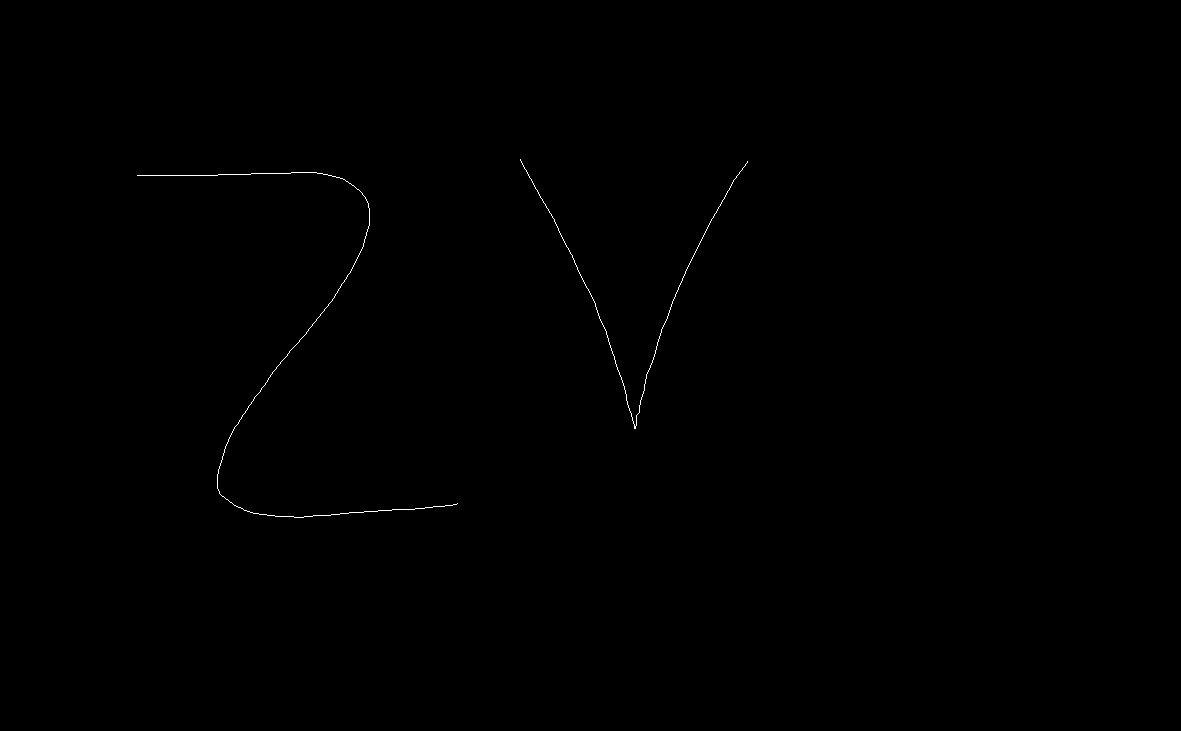
\includegraphics[width = 12cm]{image/output}
  \caption{Результат выполнения программы}
\end{figure}


% ====================================================================================================
\end{document}